%&latex
\documentclass[letterpaper]{article}
\usepackage{aaai}
\usepackage{amsfonts}
\usepackage{times}
\usepackage{helvet}
\usepackage{courier}
\usepackage{ifthen}
\usepackage{color}

\nocopyright

\newcommand{\fix}[1]{{$\langle${\sc #1}$\rangle$}}


\usepackage[pdftex]{graphicx}
\usepackage{amsmath}

\newcounter{codeline}
\newenvironment{code}{
  \newcommand{\cl}{ % code line
    \refstepcounter{codeline}
    \ifthenelse{\value{codeline}<10}{\hspace{5pt}\arabic{codeline}}{\arabic{codeline}}.
  }
  \begin{tabbing}
    00. nn\=nn\=nn\=nn\=nn\=nn\=nn\=nn\=nn\=nn\kill
} {\end{tabbing}}

% italics in math mode
\newcommand{\myit}[1]{\mbox{\em #1}}
% in subscripts
\newcommand{\myits}[1]{\mbox{\scriptsize \em #1}}

\newcommand{\citep}[1]{\citeauthor{#1}~\shortcite{#1}}
\newcommand{\citeq}[1]{\citeauthor{#1}~\citeyear{#1}}

\newcommand{\fromM}[1]{{$\langle${\sc M: #1}$\rangle$}}
\newcommand{\comment}[1]{{$\langle${\color{blue}{\sc #1}}$\rangle$}}


\newcommand{\pv}{\myit{PlanVisioner }}

% evil
\def\baselinestretch{.97}
\setlength\textheight{9.1in}
\setlength\textwidth{7.05in}
%\setlength\columnsep{0.245in}

\def\europa{{\sl EUROPA}}

\newcommand{\figwidth}[2]{\mbox{\resizebox{#1}{!}
{\includegraphics{#2}}}}

\newcommand{\fixE}[1]{$\langle${\sc EB: #1}$\rangle$}

%------------------------------
\begin{document}

\title{\europa: A Platform for Timeline-based AI Planning, Scheduling, Constraint Programming, and Optimization}

\author{\large{Javier Barreiro{$^*$}, Matthew Boyce{$^*$}, Jeremy Frank{$^\dagger$}, Michael Iatauro{$^*$}}\\
\large{\bf Paul Morris{$^\dagger$}, Tristan Smith{$^*$}, Minh Do{$^*$}}\\ \\
{\small {$^*$} SGT Inc., NASA Ames Research Center, Mail Stop 269-3, Moffett Field, CA 94035}\\
{\small {$^\dagger$} NASA Ames Research Center, Mail Stop 269-3, Moffett Field, CA 94035}
}

\date{}
\maketitle

%------
\begin{abstract}

\europa\ is a class library and tool set for building and analyzing planners within a Constraint-based Temporal Planning paradigm. This paradigm has been successfully applied in a wide range of practical planning problems and has a legacy of success in NASA applications. \europa\ offers capabilities in 3 key areas of problem solving: (1) Representation; (2) Constraint-based Reasoning; and (3) Search. \europa\ is a means to integrate advanced planning, scheduling and constraint reasoning into an end-user application and is designed to be open and extendable to accommodate diverse and highly specialized problem solving techniques within a common design framework and around a common technology core. While \europa\ is a complete tool set, in this paper, we will mostly concentrate on its timeline-based plan representation and the least-commitment partial-order planning approach operates on top of that representation.

\end{abstract}
%-----


%---------------------
\section{Introduction}


\europa\ (Extensible Universal Remote Operations Planning Architecture) is a class library and tool set for building timeline-based planners (and/or schedulers) within a Constraint-based Temporal Planning paradigm ~\cite{frank:europa}. Constraint-based Temporal Planning is a paradigm of planning based on an explicit notion of time and a deep commitment to a constraint-based formulation of planning problems. This paradigm has been successfully applied in a wide range of practical planning problems and has a legacy of success in NASA applications.

As a complete Planning \& Scheduling platform, \europa\ offers capabilities in 3 key areas of problem solving:

\begin{enumerate}
\item {\bf Representation}:  Externally, \europa's main input modeling language is the New Domain Definition Language (NDDL) (pronounced `noodle'). NDDL is a high-level object-oriented modeling language that can describe a number of concepts based on Variables and Constraints. Internally, \europa\ allows a rich representation based on \emph{durative tokens} on \emph{timelines} for actions, states, resources and constraints that allows concise declarative descriptions of problem domains and powerful expressions of plan structure.
\item {\bf Constraint-based Reasoning}: \europa's main reasoning module contains constraint-processing and inference algorithms to enforce domain rules/constraints and propagate consequences as updates are made to the problem state. Specialized techniques for reasoning about temporal quantities and relations included in \europa\ are particularly useful to deal with real-life problem domains.
\item {\bf Search}: by default, \europa\ supports chronological-backtracking search with the ability to integrate heuristics into the basic search algorithm and for developing new customized search algorithms.
\end{enumerate}


%--
\begin{figure}
  \begin{center}
    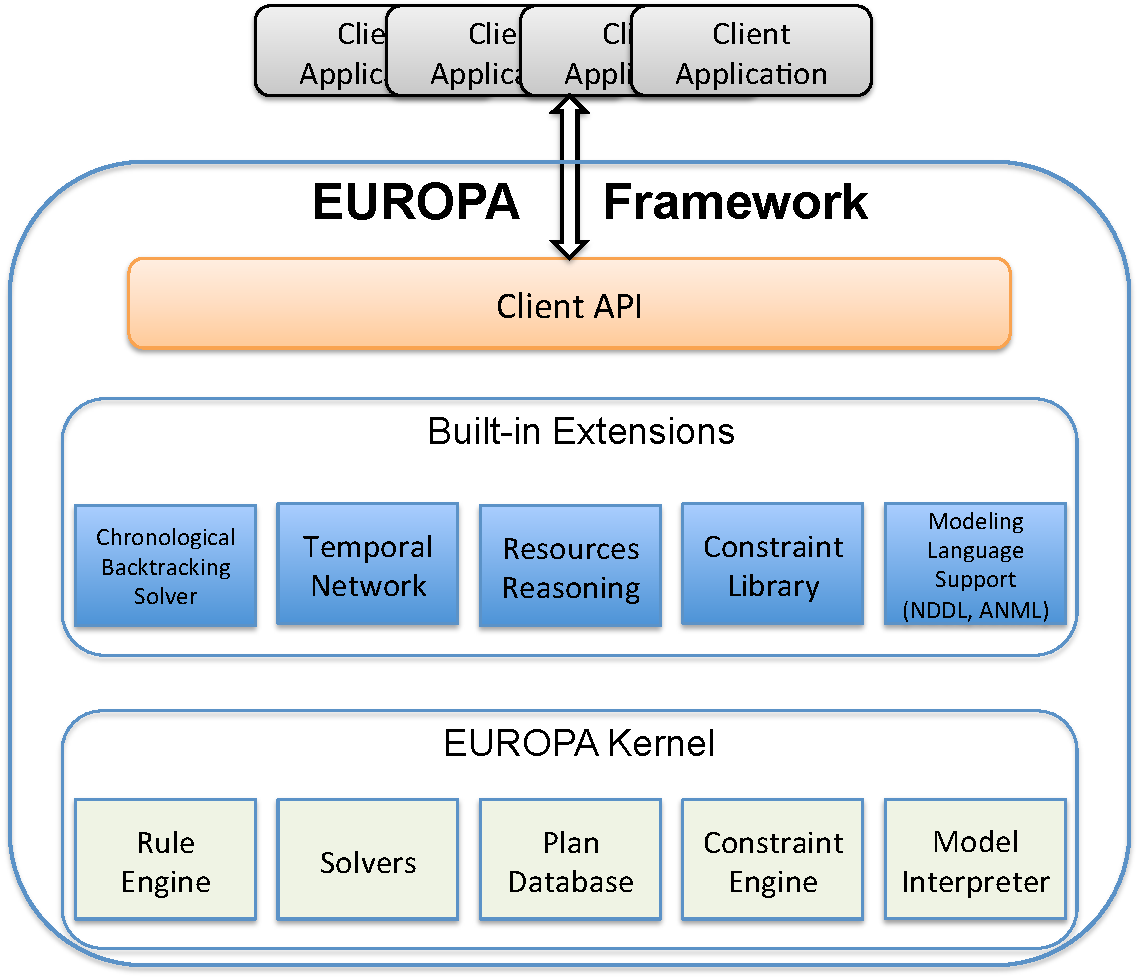
\includegraphics[width=3.4in]{EUROPA-Architecture.pdf}
  \end{center}
%	\vspace*{-0.1in}
  \caption{\small \europa\ Architecture}
  \label{fig:architecture}
%  	\vspace*{-0.1in}
\end{figure}
%--

\europa\ is designed to be open and extendable to accommodate diverse and highly specialized problem solving techniques within a common design framework and around a common technology core. Figure~\ref{fig:architecture} shows the main components of \europa\ and the hierarchical relationships between them: through the \emph{Client API}, applications can utilize or extend either the core components of the \emph{\europa\ kernel} or the built-in commonly used components that are extensions of the kernel components. \europa\ is now at version 2.6 which embodies significant evolution from the original \europa, which in turn was based upon HSTS ~\cite{muscettola:1998}. It has been made available under an open-source license. The source code and extensive documents on \europa\ are available at: \emph{http://code.google.com/p/europa\-pso/}. 


%----------
\section{Timeline-based Planning}

\noindent {\bf Modeling:} The NDDL input modeling language representation includes state and activity descriptions, as is common in planners using traditional modeling languages like the Planning Domain Definition Language (PDDL) that support the variable-value formalism. \europa\ thus takes its heritage from planning formalisms like IxTeT and SAS+. The NDDL models are parsed/translated into an internal representation with the following core components:

\begin{itemize}
\item {\bf Timeline \& Token:} \europa\ state variables are represented using \emph{timelines}, and the changing values on timelines represent sequences of states. Specifically, states are represented as a set of temporally extended predicates called \emph{tokens} and the temporal and logical constraints between them. Each token consists of a proposition and a list of parameters, which by default includes the \emph{start}, \emph{end} and \emph{duration} temporal variables.  Timelines consist of totally ordered sequences of connected tokens; hence, a timeline can be in only one state at any instant. Note that while tokens mostly represent temporally-extended predicates, which resemble world-state, tokens also represent actions in \europa\ and thus may not be on some particular timelines.
\item {\bf Compatibility:} The final component of NDDL model is a set of compatibilities/rules that govern the legal arrangements of states on, and across, timelines.  These compatibilities are logical implications asserting that if a timeline is in a state (represented by a given token), then other timelines must be in one of a set of compatible states. Compatibilities can incorporate (1) explicit logical and arithmetic constraints on the parameters of the states/tokens or (2) temporal constraints between tokens.  \europa\ provides a library of such constraints (e.g., all of the Allen's Temporal Relations), and this library can be extended if new constraints are needed.
\end{itemize}

\noindent{\bf Least-Commitment Partial Planning Refinement Search:} EUROPA follows the \emph{lifted plan-space refinement} planning approach. It uses a series of refinements to convert an initial partial plan into a final plan that is complete with respect to the requirements of the planner. A partial plan consists of a set of timelines containing a partially instantiated and ordered set of tokens with the possible flaws of: (1) unbound variables; (2) open condition; and (3) temporal threats.  Flaws are resolved one at a time following user-defined flaw filter and flaw selection strategy and a complete plan is returned when there are no flaws. The main flaw types and the resolution strategy for each of them are:

\begin{itemize}
\item {\bf Unbound Variable:} a variable in the partial plan whose domain is not a singleton. A unbound variable flaw is resolved by specifying a value from the domain of that variable.
\item {\bf Open Condition:} when a new token is added to the partial-plan, its status is \emph{inactive} and it represents an open-condition flaw. This type of flaw can be resolved by: (1) \emph{merge} with an existing active token; (2) \emph{activate} and add to timeline; or (3) \emph{reject} (if this option is allowed for the flawed token). When a token is ``activated", it can introduce a new set of (inactive) \emph{slave} tokens. For example, if the activated token represents a durative action, then (slave) tokens representing (pre)conditions and effects are added as new inactive tokens (new open conditions).
\item {\bf Threat:} once a token has been placed in the partial plan it may impact other tokens indirectly through possible overlapping requirements on objects, or by creating resource oversubscription. Threats are resolved by imposing ordering constraints among tokens.
\end{itemize}

There are extendable built-in flaw-filter and flaw-selection strategies to decide which flaw to be handled next. For the built-in chronological backtracking (depth-first) search solver, when a flaw is selected, it represents a branching point in the search graph with the next child search node to be selected/explored basing on the resolution-selection strategy (which \europa\ also provides extendable built-in options). The flaw-resolution strategy is backed by strong constraint propagation routines with special emphasis on temporal and resource reasoning.The search process stops when there is no additional flaw to handle. The built-in solver is only one of many search strategies that can be implemented using \europa\, all of the solver components are designed to allow the \europa\ user to implement other search algorithms and heuristics as required by the problem domain being addressed.

%---------
\section{Current State \& Future Work}

\europa\ and its supporting tools have been going through a long period of development. Besides the core modeling and reasoning capabilities, \europa\ also provides a streamlined API to integrate with native client applications, Eclipse's plugins to help build and debug NDDL/ANML models, and visualization capabilities to support plan comprehension and diagnosis. Overall, \europa's current main strengths include: (1) proven track record of addressing real life planning and schedulingproblems; (2) expressive modeling capability; (3) flexible framework; (4) strong support for integration with other applications; (5) open-source license. It has been used for a variety of missions, mission-oriented research, and demonstrations, including: DS1: RAX �Remote Agent Experiment, Support for operation of the International Space Station's solar arrays, Bedrest study at Johnson Space Center, MER Tactical Activity Planning, Advanced Spaceflight Training Systems Development, MBARI's underwater autonomous vehicle, and Willow Garage's autonomous robot navigation.

Nevertheless, we still have a long list of improvements for \europa. The most important ones in our opinion are: significant improvements for search (especially heuristic guidance) and inference capabilities, support the ANML and PDDL modeling languages, improve the visualization and debugging tools and  allow \europa\ extensions to be written in other languages. Given that \europa\ is open-source software, we welcome contributions from planning and scheduling researchers and practitioners.




{\small
\bibliography{/Users/mbdo/Documents/master}
\bibliographystyle{aaai}
}




\end{document}



%EOF